\documentclass[tikz,multi=false,border=5mm]{standalone}
\usetikzlibrary{arrows}

\begin{document}

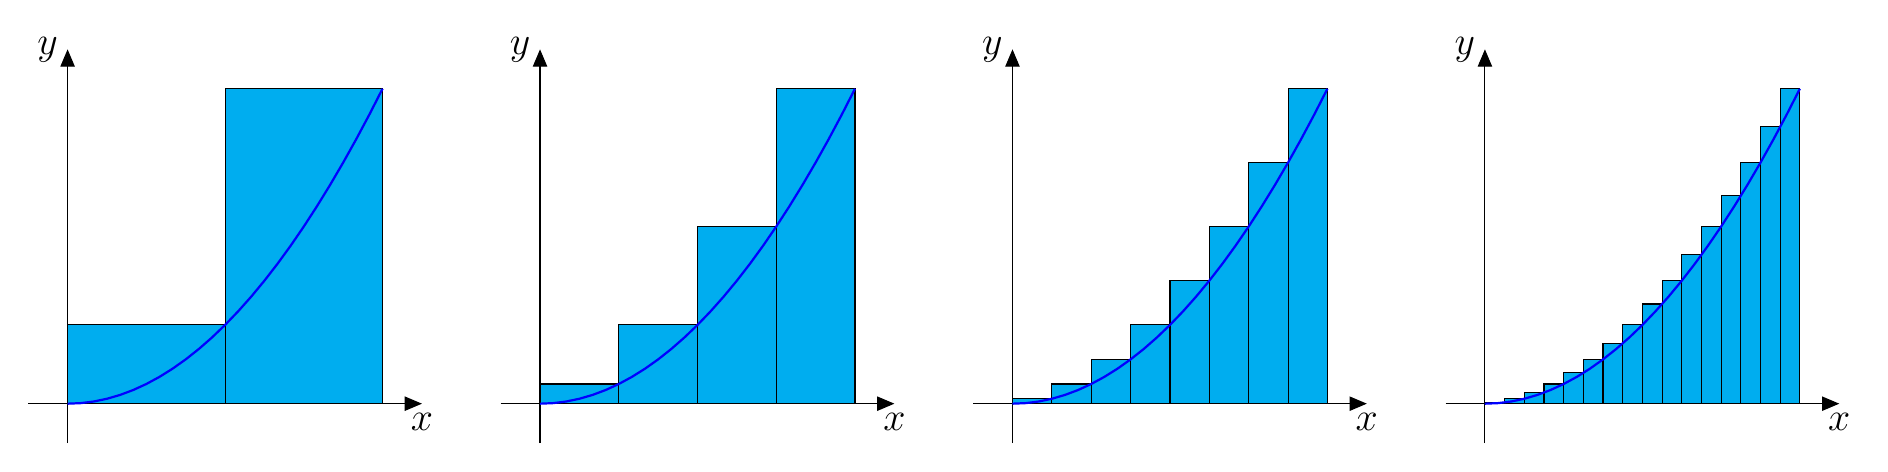
\begin{tikzpicture}
\foreach \i/\p/\a in {0/2/2,1/1/3,2/.5/3.5,3/.25/3.75} {%
  \begin{scope}[xshift=6*\i cm,>=triangle 45]
  \foreach \x in {0,\p,...,\a} {%
    \draw[fill=cyan] (\x,0) -- (\x,{.25*pow(\x+\p,2)}) -- (\x+\p,{.25*pow(\x+\p,2)}) -- (\x+\p,0);
    %\draw[fill=orange] (\x,0) -- (\x,.25*\x*\x) -- (\x+\p,.25*\x*\x) -- (\x+\p,0);
  }
  \draw [->] (-.5,0) -- ++(5,0) node[below] {\Large $x$};
  \draw [->] (0,-.5) -- ++(0,5) node[left] {\Large $y$};
  \draw [thick,blue,domain=0:4] plot (\x,{.25*pow(\x,2)});
  \end{scope}
}
\end{tikzpicture}

\end{document}